\documentclass[12pt]{article}
\usepackage{amsmath}
\usepackage{mathtools}
\usepackage{bigints}
\usepackage{parskip}
\usepackage{amssymb}
\usepackage{relsize}
\usepackage{fullpage}
% \DeclareMathSizes{12}{17.28}{9}{7} % (a)

\DeclareMathSizes{12}{17.28}{12}{12} % (a)


\usepackage{hyperref}



	\addtolength{\topmargin}{-.5in}
	\addtolength{\textheight}{1.75in}



    \newenvironment{myindentpar}[1]%
     {\begin{list}{}%
             {\setlength{\leftmargin}{#1}}%
             \item[]%
     }
     {\end{list}}

\begin{document}
\title{College Algebra: Module 12 What You Need To Know}
\date{3-28-15}
\author{}
\maketitle

\section{Logarithms and Logarithmic Functions (Section 5.3)}

\textbf{Logarithm Function}
\newline

\centerline{$f(x) = \log_{b}(x)$ \hspace{2cm} $b \neq 1$ and $b > 0$} 

\vspace{.5cm}

\centerline{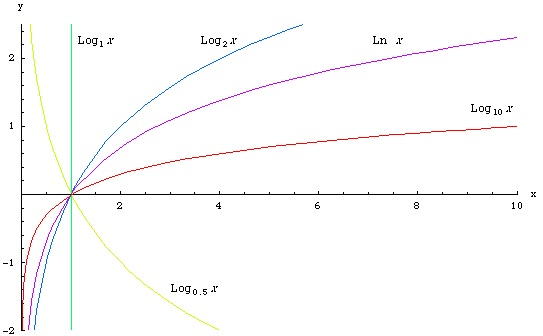
\includegraphics{LogGraph.jpg}}

We call $b$ the \textbf{base} of the logarithm function. 

There is a special kind of logarithm function that we single out becaue of its significance. It is the \textbf{Natural Log Function}. It is the function
\newline

\centerline{$f(x) = \ln(x)$}

The Natural Log Function is the logarithm function with \textbf{base e}:
\newline

\centerline{$f(x) = \log_{e}(x) = \ln(x)$}

and it is the \textbf{inverse} of the natural exponential function $f(x) = e^{x}$

\textbf{Note:} If you see something like $f(x) = \log(x)$ with no base, then we assume it is \textbf{log base 10}, or written out, we assume $f(x) = \log_{10}(x)$

\vspace{1cm}

\textbf{Logarithm to Exponential Conversion:}
\newline

\centerline{$y = \text{log}_{b}(x) \Leftrightarrow x = b^{y}$}

\vspace{1cm}

\textbf{Finding Domain of a Log Function:}
\newline

\centerline{Given $\text{log}_{b}(\text{STUFF})$ we set STUFF $> 0$}


\begin{myindentpar}{1cm}
\textbf{Example:} Find the domain of $\text{log}_{3}(x-3)$

\begin{myindentpar}{2cm}
- Set $x - 3 > 0 \implies x > 3$ is the domain
\end{myindentpar}
\end{myindentpar}

\section{Properties of Logarithms (Section 5.4)}

\textbf{Important Properties of Logs:}
\begin{myindentpar}{2cm}
\begin{enumerate}
\item $\log_{b}(1) = 0$
\item $\log_{b}(b) = 1$
\item $\log_{b}(b^{x})= x$
\item $b^{\log_{b}(x)} = x$
\item $\log_{b}(x \cdot y) = \log_{b}(x) + \log_{b}(y)$ 
\item $\log_{b}\Big(\dfrac{x}{y}\Big) = \log_{b}(x) - \log_{b}(y)$
\item $\log_{b}(x^{p}) = p \cdot \log_{b}(x)$
\end{enumerate}
\end{myindentpar}

\vspace{1cm}

\textbf{Change of Base:}
\newline

\centerline{$\log_{b}(M) = \dfrac{\log_{a}(M)}{\log_{a}(b)}$}



























\end{document}